\subsection{Bolometric IR Luminosity Density} \label{Sec: IR Density}
In this section, we calculate and analyse the bolometric IR (8-1000$\mu$m) luminosity density (LD) and star formation rate density ($\rho_{SFRD}$). Figure \ref{Fig: SFRD} shows the IR LD ($\rho_{IR}$) of our ZFOURGE and CIGALE results with values in table \ref{Tab: SFRD}. At each redshift bin, $\rho_{IR}$ is calculated by integrating under the best fitting luminosity function with equation \ref{EQ: Luminosity Density}. Where $\phi(L)$ is the best fitting luminosity function (in our case, the Schechter or Saunders function: equations \ref{EQ: Shechter Function} and \ref{EQ: Saunders Function} respectively). Schechter is used for the CIGALE SF, whereas Saunders is used for ZFOURGE total and CIGALE AGN. We utilise \texttt{scipy.integrate.quad} \citep{virtanen_scipy_2020} to perform the integration from $0$ to $\infty$ $L_{\odot}$ by cumulatively summing the integrand at incremental bounds (e.g. from $10^{10}$ to $10^{12}$ $L_{\odot}$, $10^{12}$ to $10^{14}$ $L_{\odot}$, etc) because the quadrature algorithm isn't well suited for small areas over very large bounds. In practice, additional calculations of $\rho_{IR}$ above $10^{20}$ $L_{\odot}$ are negligible. To generate $1\sigma$ $\rho_{IR}$ uncertainties, we re-perform the integration using the $1 \sigma$ LF fit errors.

\begin{equation} 
    \rho_{IR} = \frac{1}{\ln(10)} \int_{0}^{\infty} \varphi(L) dL 
    \label{EQ: Luminosity Density}
\end{equation}

\begin{table}
    \begin{center}
    \caption{Luminosity density as a function of redshift. Units are in log($\rho_{IR}$) [$L_{\odot}$ Mpc$^{-3}$]. Errors are absolute. $\rho_{IR}$ values are centered on the redshift bin.}
    \label{Tab: SFRD}
    \begin{tabular}{@{}cccc@{}}
        \toprule
        $z$ & ZFOURGE Total & CIGALE SF & CIGALE AGN \\
        \hline
        0.00 $\leq z <$ 0.30 & 7.98$^{0.27}_{0.21}$ & 8.58$^{0.19}_{0.16}$  & 7.53$^{0.80}_{0.37}$ \\
        0.30 $\leq z <$ 0.45 & 8.24$^{0.49}_{0.32}$ & 8.50$^{0.21}_{0.18}$  & 7.81$^{0.73}_{0.40}$ \\
        0.45 $\leq z <$ 0.60 & 8.38$^{0.16}_{0.14}$ & 8.62$^{0.17}_{0.15}$  & 7.62$^{0.29}_{0.23}$ \\
        0.60 $\leq z <$ 0.80 & 8.72$^{0.19}_{0.16}$ & 9.04 $\pm$ 0.01       & 7.70$^{0.26}_{0.21}$ \\
        0.80 $\leq z <$ 1.00 & 8.79$^{0.22}_{0.18}$ & 9.20 $\pm$ 0.01       & 7.80$^{0.46}_{0.31}$ \\
        1.00 $\leq z <$ 1.20 & 8.72$^{0.30}_{0.23}$ & 8.99 $\pm$ 0.02       & 7.85$^{0.28}_{0.22}$ \\
        1.20 $\leq z <$ 1.70 & 8.98$^{0.09}_{0.08}$ & 9.28 $\pm$ 0.02       & 8.20$^{0.45}_{0.31}$ \\
        1.70 $\leq z <$ 2.00 & 9.27 $\pm$ 0.02      & 9.52 $\pm$ 0.03       & 8.47$^{0.26}_{0.21}$ \\
        2.00 $\leq z <$ 2.50 & 9.07$^{0.13}_{0.12}$ & 9.45 $\pm$ 0.03       & 8.46$^{0.36}_{0.26}$ \\
        2.50 $\leq z <$ 3.00 & 9.16 $\pm$ 0.03      & 9.22 $\pm$ 0.02       & 8.47$^{0.12}_{0.11}$ \\
        3.00 $\leq z <$ 4.20 & 9.38 $\pm$ 0.04      & 8.78 $\pm$ 0.01       & 8.37$^{0.21}_{0.17}$ \\
        4.20 $\leq z <$ 6.00 & 9.12 $\pm$ 0.08      & 8.28 $\pm$ 0.02       & 7.91 $\pm$ 0.07 \\
        \bottomrule
    \end{tabular}
    \end{center}        
\end{table}

\begin{figure*}
    \centering
    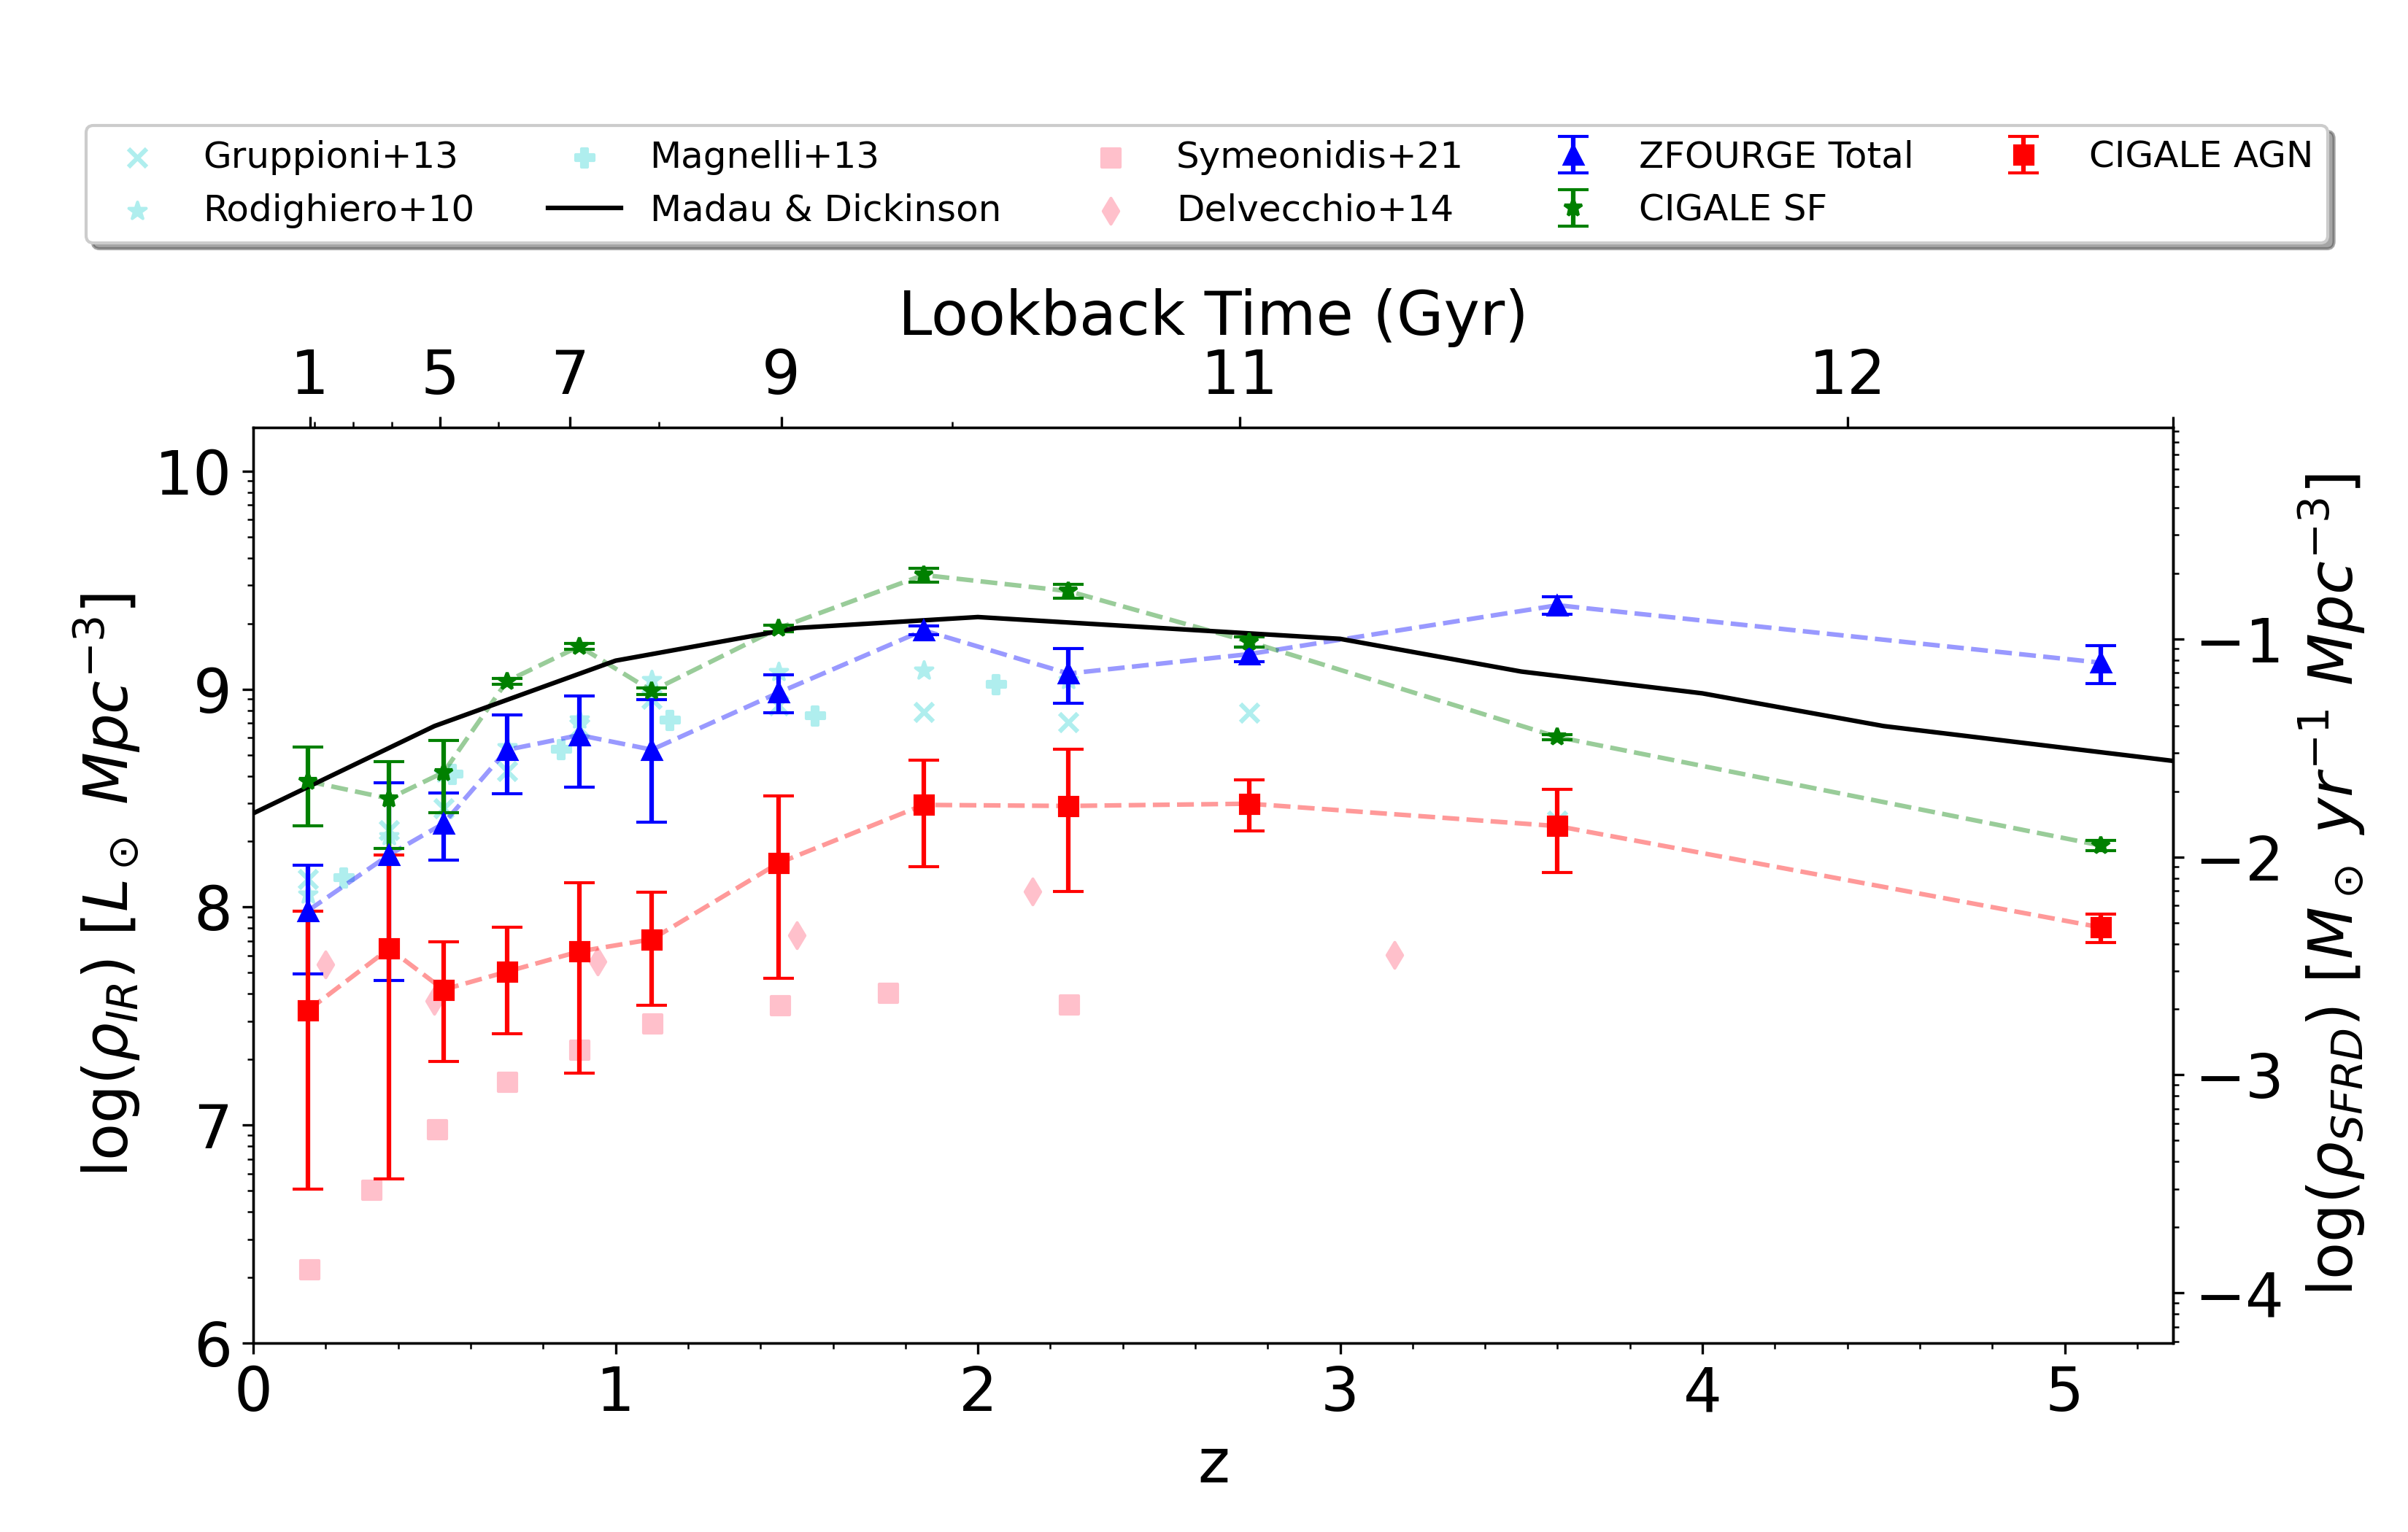
\includegraphics[width=\textwidth]{Figures/SFRD.png}
    \caption{Evolution of the IR luminosity density (LD) calculated by integrating under the best fitting LFs. $1\sigma$ uncertainties are calculated by re-performing the integration with errors from the LF fitting process. Saunders is fit for the ZFOURGE total and CIALE AGN, whereas Schechter is fit for the CIGALE SF. Blue triangles represent ZFOURGE total; green stars CIGALE SF; and red squares CIGALE AGN. The right side y-axis is obtained from \cite{kennicutt_global_1998} with $\rho_{SFRD} = \rho_{IR} \times 1.7\times10^{-10} \ L_{\odot}$. The top axis shows the lookback time in billions of years. We compare our results with relevant literature. \cite{gruppioni_herschel_2013, rodighiero_mid-_2010, magnelli_deepest_2013} as light blue compare the SF LD. \cite{symeonidis_agn_2021} and \cite{delvecchio_tracing_2014} as light red compare the AGN LD. The solid black line is the \cite{madau_cosmic_2014} LD.}
    \label{Fig: SFRD}
\end{figure*}

\begin{figure*}
    \centering
    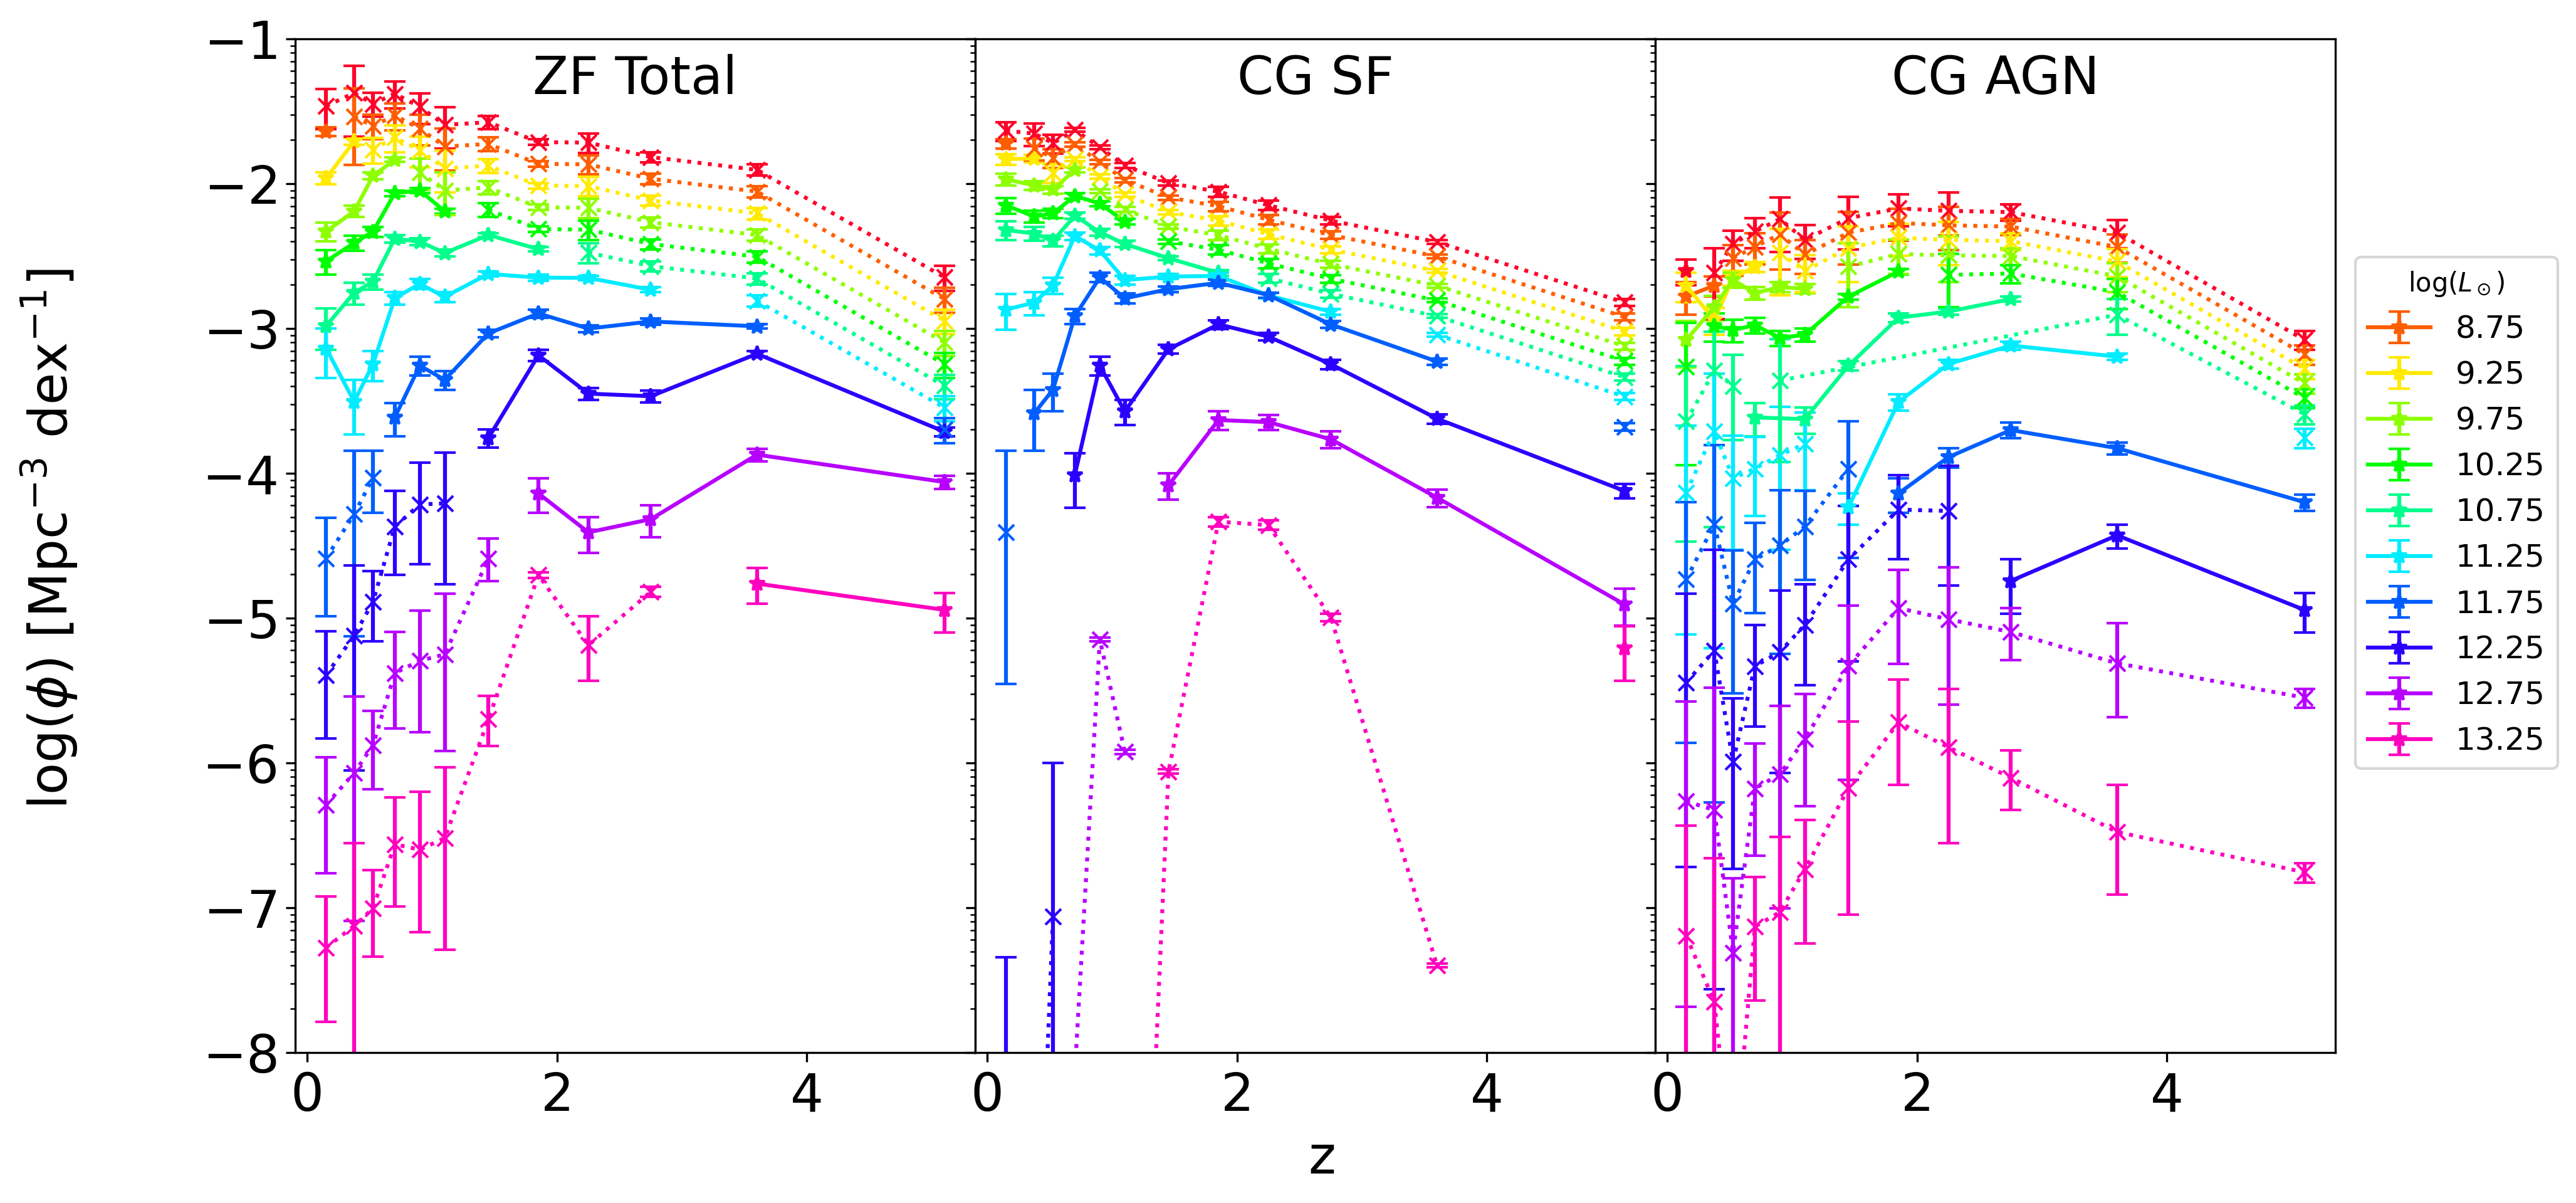
\includegraphics[width=\textwidth]{Figures/Class_Evo.png}
    \caption{Luminosity class evolution as a function of redshift. $\phi$ values connected by straight lines correspond to real calculated values. $\phi$ values connected by dotted lines are estimated from the best fitting function (Schechter for CIGALE SF, Saunders for ZFOURGE Total and CIGALE AGN). Error bars represent the 1$\sigma$ uncertainty calculated with equation \ref{EQ: Vmax Error} for real values or derived from the function fitting process for estimated values. Real luminosity classes are 0.5 log$(L_{\odot})$ in width and centred in the middle (e.g. 8.5 --- 9.0 is centred on 8.75). Estimated classes are calculated at the centre of the luminosity bin (e.g. 8.75).}
    \label{Fig: Class Evo}
\end{figure*}

The secondary right-hand-side axis of figure \ref{Fig: SFRD} displays the conversion to SFRD provided by \cite{kennicutt_global_1998} calculated with $\rho_{SFRD} = \rho_{IR} \times 1.7\times10^{-10} L_{\odot}$. We remind the reader that the IR AGN densities do not have an associated SFR. The top x-axis shows the lookback time in billions of years, placing the evolution of the universe in the context of time to showcase the important evolutionary epochs.

Our ZFOURGE results in figure \ref{Fig: SFRD} show rapid evolution from $0<z<2$. From $z>2$ onwards, there is essentially no evolution. As discussed in section \ref{Sec: Parameter Evolution}, our highest redshift bin was thought to suffer from incompleteness, but our $\rho_{IR}$ results do not obviously show it. We see excellent agreement with the literature from $0<z<2$ but deviate significantly from $z>2$ onwards. Importantly, we do not find a turnover in the IR LD at $z\approx2$. This is a different result than is often published in the literature (\citealp{gruppioni_herschel_2013, magnelli_deepest_2013, madau_cosmic_2014, lutz_far-infrared_2014} and references within). However, this is not a new result as is seen in \cite{rodighiero_mid-_2010}, but they do not probe to a sufficiently high enough redshift to capture the decline above $z>2$.

The CIGALE decomposed SF IR LD is seen to increase from $0<z<2$ and decline from $z>2$ onwards. This agrees well with the literature, especially \cite{madau_cosmic_2014}. The ability of CIGALE to recover the turnover in the SF IR LD, where ZFOURGE does not, suggests that CIGALE is effectively isolating the SF component and lends confidence to the accuracy of our results. The CIGALE SF LD is slightly elevated over ZFOURGE at most redshift bins. We believe this is not an error on CIGALE's part or the ZFOURGE data it is based on, but a representation of the true pure SF IR LD because AGN contaminants have been effectively eliminated. As mentioned previously in section \ref{Sec: Bolometric IR LF}, both \cite{fu_decomposing_2010} and \cite{wu_mid-infrared_2011} argue that when AGN are removed, the luminosity function is better fit with a Schechter function. This agrees with our results and explains why our CIGALE SF LFs (figure \ref{Fig: Bolometric IR LF}) are elevated. Integrating under the CIGALE SF Schechter functions, we see an elevation in $\rho_{IR}$. 

The CIGALE AGN LD follows a similar evolution to the literature, though it is elevated, likely due to CIGALE's ability to detect fainter AGN. The trend seen in the CIGALE SF LD increasing from $0<z<2$ and declining from $z>2$ is still present in the AGN LD. This is not the first time a turnover in the AGN $\rho_{IR}$ has been seen. \cite{symeonidis_agn_2021} presents their IR AGN densities up to $z\approx2.5$. These results are at most $\approx 1$ order of magnitude lower than ours. We attribute this to their use of \cite{aird_evolution_2015} X-ray sources, which are converted to optical luminosity and then to IR luminosity. Their X-ray-selected galaxies likely miss the highly obscured and faint-luminosity counterpart that this work recovers. As \cite{symeonidis_agn_2021} only extends as far as $z\approx2.5$, the AGN $\rho_{IR}$ turnover is not well defined. AGN by \cite{delvecchio_tracing_2014} agrees well with our results. We recalculated the AGN $\rho_{IR}$ for the \cite{delvecchio_tracing_2014} dataset because they did not provide $\rho_{IR}$ values in their work, instead focusing on the black hole accretion rate density ($\Psi_{bhar}$). Using the function parameters they reported, we use the same integration method described previously to calculate $\rho_{IR}$.

Both \cite{symeonidis_agn_2021} and \cite{delvecchio_tracing_2014} show AGN LD peaks at $z\approx2$ whereas our CIGALE AGN LD peaks sometime between $z\approx2-3$. As was mentioned in section \ref{Sec: Parameter Evolution}, there appeared to be a significant evolutionary epoch for AGN occurring at $z\approx1$. Despite the parameter evolution (Figure \ref{Fig: Param Evo}) seemingly hinting at a significant cosmic epoch for AGN evolution, we do not obviously see this reflected in our AGN LD results. From $0<z<2$, AGN density is seen to decline, albeit slowly and with some scatter. Our two lowest redshift bins have high uncertainties, so there remains the possibility that somewhere between $0<z<1$ is a significant time for AGN evolution. Therefore, relying solely on the LD evolution of AGN and SF galaxies to assess their overall evolution may oversimplify their complex evolution. The functional fits smoothed out slight variations in the LF, potentially masking essential details.